\documentclass[12pt,a4paper]{article}
\raggedbottom

\usepackage{ugmath}
\usepackage{float}
\usepackage{placeins}
\usepackage[labelfont=bf,labelsep=space]{caption}
\usepackage{pdfpages}
\usepackage{tikz-cd}
\usepackage{amsthm}
\renewcommand{\Tr}{\operatorname{Tr}}
\newcommand{\llaves}[1]{\{#1\}}
\newcommand{\parentesis}[1]{\left(#1\right)}
\newcommand{\corchetes}[1]{\left[#1\right]}
\newcommand{\llavesgrande}[1]{\big\{#1\big\}}
\newcommand{\llavesgrandes}[1]{\left\{#1\right\}}


\begin{document}

    \thispagestyle{empty}
    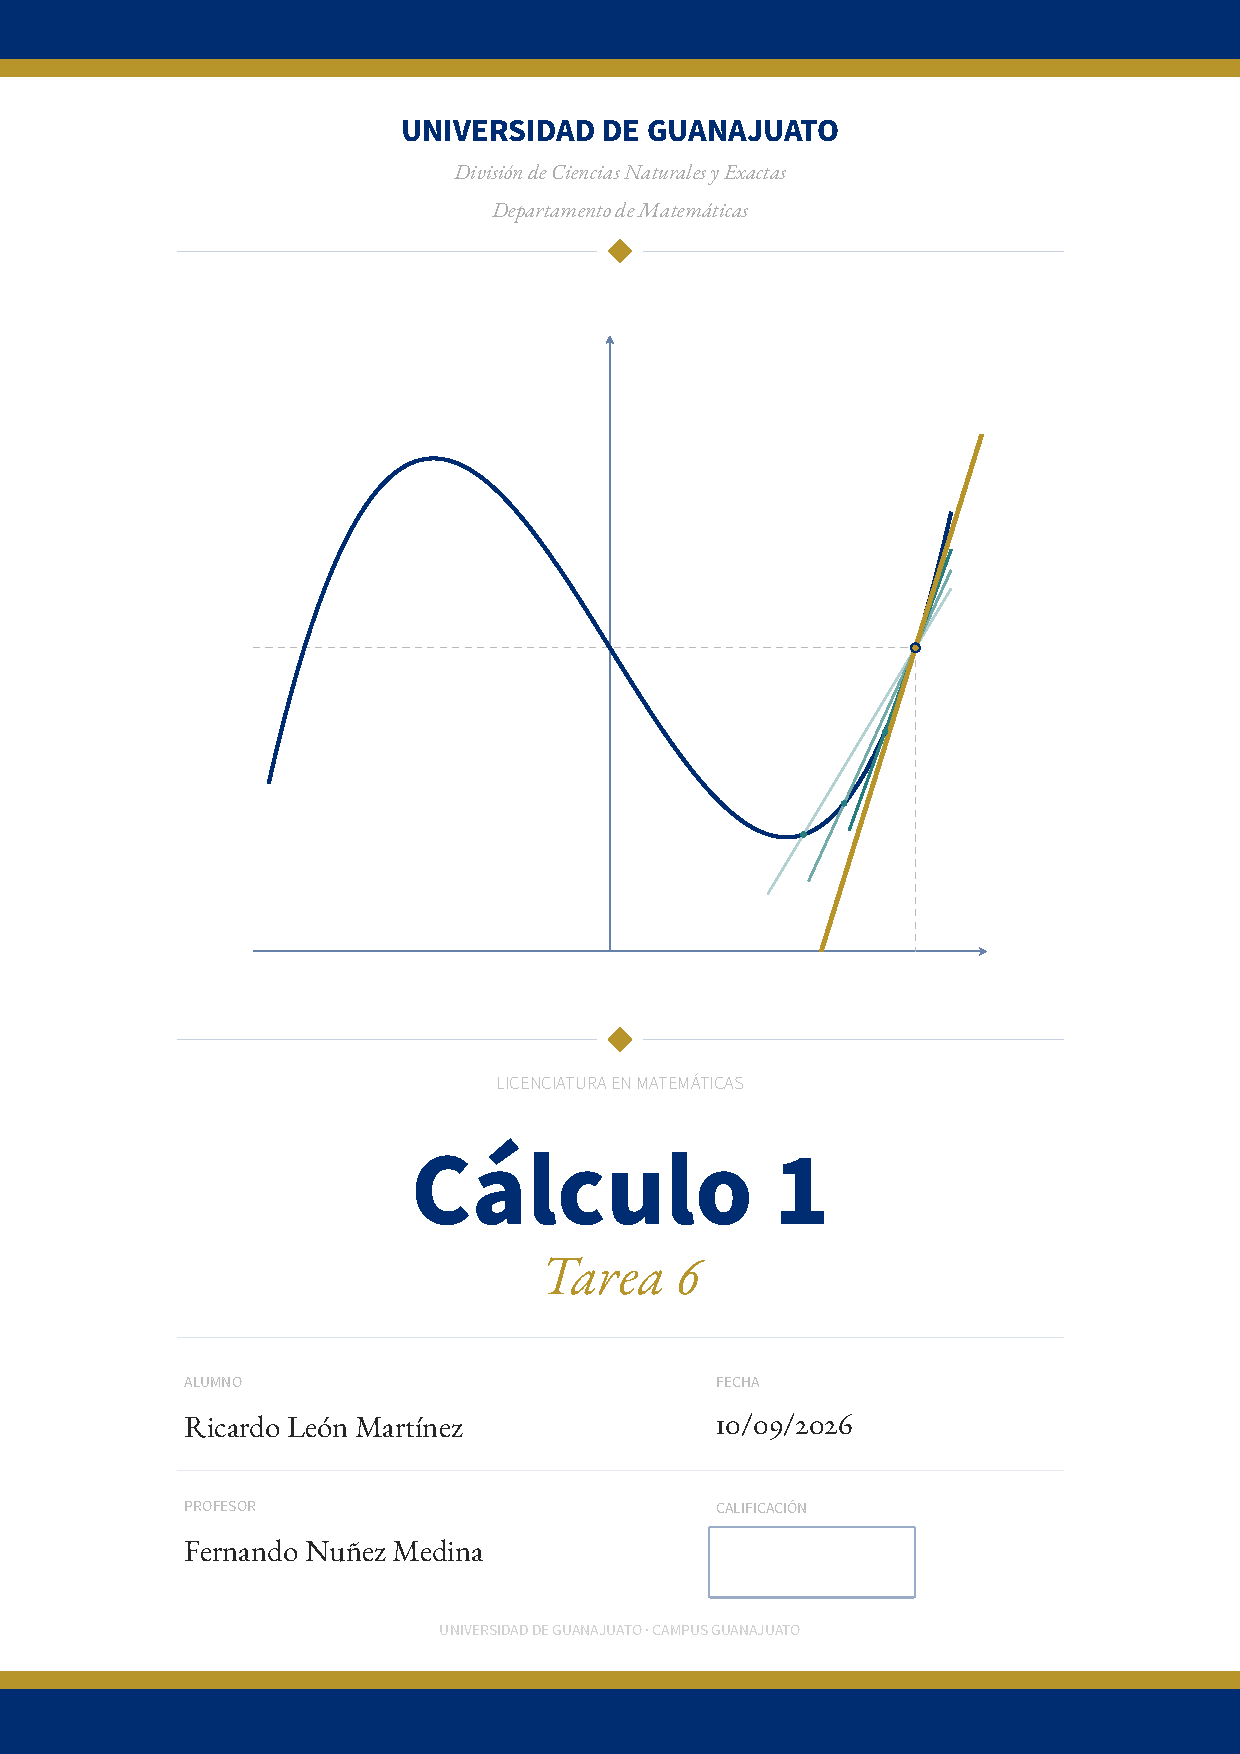
\includepdf[pages=1]{main.pdf}

    \begin{problema}
        \textbf{(Potencias enteras negativas)} Sean $x\neq0$ y $n$ un número natural. Usa la unicidad del inverso multiplicativo para probar que
        \begin{equation*}
            \left(x^{n}\right)^{-1}=\left(x^{-1}\right)^{n}.
        \end{equation*}
        En vista de esta ecuación se define $x^{-n}$ como $\left(x^{n}\right)^{-1}$ o como $\left(x^{-1}\right)^{n}$.
    \end{problema}

    \begin{proof}
        Por el inciso (c) de las leyes de los exponentes, que es el ejercicio 22, si $y\in\R$, entonces $x^{n}y^{n}=(xy)^{n}$. Tomando $y=x^{-1}$ y usando el axioma 8 obtenemos
        \begin{equation*}
            x^{n}\left(x^{-1}\right)^{n}=\left(x\cdot x^{-1}\right)^{n}=1^{n}=1,
        \end{equation*}
        donde $1^{n}=1$, pues $1^{n}$ es el producto de $1$ consigo mismo $n$ veces por la definición 11 y $1\cdot1=1$ por el axioma 7.
        Notemos que $x^{n}\neq0$, pues si $x^{n}=0$, la igualdad anterior y la proposición 7 darían $1=0\cdot\left(x^{-1}\right)^{n}=0$, lo cual es imposible, pues $1\neq0$ por el axioma 7. Así, $x^{n}$ tiene inverso multiplicativo, y la igualdad anterior dice que $\left(x^{-1}\right)^{n}$ cumple la propiedad del inverso multiplicativo de $x^{n}$. Por la unicidad del inverso multiplicativo, que es el inciso (b) de la proposición 6, concluimos que
        \begin{equation*}
            \left(x^{n}\right)^{-1}=\left(x^{-1}\right)^{n}.\qedhere
        \end{equation*}
    \end{proof}

    \begin{problema}
        Prueba que $1>0$. \textbf{Sugerencia:} Considera la proposición 11.
    \end{problema}

    \begin{proof}
        Por la proposición 11, para todo número real $x\neq0$ se cumple que
        \begin{equation*}
            x^{2}>0.
        \end{equation*}
        Por el axioma 7, $1$ es un número real distinto de $0$, así que podemos tomar $x=1$. Además, por el mismo axioma con $x=1$, se tiene $1^{2}=1\cdot1=1$. Por lo tanto,
        \begin{equation*}
            1=1^{2}>0.\qedhere
        \end{equation*}
    \end{proof}

    \begin{problema}
        Sean $A$ un subconjunto de números reales y $c\in\R$. Definimos
        \begin{equation*}
            cA=\left\{ ca:a\in A\right\} .
        \end{equation*}
        Prueba que si $A$ es no vacío y acotado superiormente, y $c\geq0$, entonces
        \begin{equation*}
            \sup\left(cA\right)=c\sup\left(A\right).
        \end{equation*}
    \end{problema}

    \begin{proof}
        Como $A$ es no vacío y acotado superiormente, por el axioma del supremo existe $\sup(A)\in\R$. Distinguimos dos casos.
        \textbf{Caso $c=0$.} Como $A\neq\varnothing$, por la proposición 7 se tiene $cA=\{0\cdot a:a\in A\}=\{0\}$, cuyo máximo, y por lo tanto supremo, es $0$. Por lo tanto,
        \begin{equation*}
            \sup(cA)=0=0\cdot\sup(A)=c\sup(A).
        \end{equation*}
        \textbf{Caso $c>0$.} Primero veamos que $c\sup(A)$ es una cota superior de $cA$. Sea $y\in cA$. Entonces $y=ca$ para algún $a\in A$. Como $a\leq\sup(A)$ y $c>0$, por la preservación del orden bajo el producto por números positivos,
        \begin{equation*}
            y=ca\leq c\sup(A).
        \end{equation*}
        Así, $c\sup(A)$ es una cota superior de $cA$.
        Ahora veamos que $c\sup(A)$ es la mínima cota superior de $cA$. Sea $C$ una cota superior de $cA$ y supongamos que $C<c\sup(A)$. Entonces
        \begin{equation*}
            \e=\sup(A)-\frac{C}{c}>0,
        \end{equation*}
        así que, por la proposición 13, existe $a\in A$ tal que $\sup(A)-\e<a$, es decir, $C/c<a$. Multiplicando por $c>0$ obtenemos
        \begin{equation*}
            C<ca.
        \end{equation*}
        Como $ca\in cA$, esto contradice que $C$ es cota superior de $cA$. Por lo tanto, $c\sup(A)\leq C$ para toda cota superior $C$ de $cA$, es decir, $c\sup(A)$ es la mínima cota superior de $cA$. Por la definición 15 de supremo,
        \begin{equation*}
            \sup(cA)=c\sup(A).\qedhere
        \end{equation*}
    \end{proof}

    \begin{problema}
        \textbf{(Binomio de Newton)} Sean $a$ y $b$ números reales y $n$ un número natural. Prueba que
        \begin{equation*}
            (a+b)^{n}=\binom{n}{0}a^{n}+\binom{n}{1}a^{n-1}b+\cdots+\binom{n}{n-1}ab^{n-1}+\binom{n}{n}b^{n}.
        \end{equation*}
        \textbf{Sugerencia:} Usa el principio de inducción matemática y ten presente el ejercicio 4 de la tarea 5.
    \end{problema}

    \begin{proof}
        En notación de suma, queremos probar que, para todo $n\in\N$,
        \begin{equation*}
            (a+b)^{n}=\sum_{k=0}^{n}\binom{n}{k}a^{n-k}b^{k}.
        \end{equation*}
        Usaremos el principio de inducción matemática, que es la proposición 15.
        \textbf{Caso base ($n=1$).} Por el ejercicio 4(a) de la tarea 5, $\binom{1}{0}=\binom{1}{1}=1$, así que
        \begin{equation*}
            \sum_{k=0}^{1}\binom{1}{k}a^{1-k}b^{k}=\binom{1}{0}a+\binom{1}{1}b=a+b=(a+b)^{1}.
        \end{equation*}
        \textbf{Paso inductivo.} Supongamos que la fórmula es válida para algún $n\in\N$. Entonces, por la hipótesis de inducción y la distributividad,
        \begin{align*}
            (a+b)^{n+1}&=(a+b)^{n}(a+b)\\
            &=\left(\sum_{k=0}^{n}\binom{n}{k}a^{n-k}b^{k}\right)(a+b)\\
            &=\sum_{k=0}^{n}\binom{n}{k}a^{n+1-k}b^{k}+\sum_{k=0}^{n}\binom{n}{k}a^{n-k}b^{k+1}.
        \end{align*}
        En la segunda suma hacemos el cambio de índice $j=k+1$, de modo que $j$ va de $1$ a $n+1$ y $n-k=(n+1)-j$:
        \begin{equation*}
            \sum_{k=0}^{n}\binom{n}{k}a^{n-k}b^{k+1}=\sum_{j=1}^{n+1}\binom{n}{j-1}a^{(n+1)-j}b^{j}.
        \end{equation*}
        Renombrando $j$ como $k$ y separando el término $k=0$ de la primera suma y el término $k=n+1$ de la segunda, obtenemos
        \begin{align*}
            (a+b)^{n+1}&=\binom{n}{0}a^{n+1}+\sum_{k=1}^{n}\binom{n}{k}a^{n+1-k}b^{k}+\sum_{k=1}^{n}\binom{n}{k-1}a^{n+1-k}b^{k}+\binom{n}{n}b^{n+1}\\
            &=a^{n+1}+\sum_{k=1}^{n}\left[\binom{n}{k-1}+\binom{n}{k}\right]a^{n+1-k}b^{k}+b^{n+1},
        \end{align*}
        donde usamos que $\binom{n}{0}=\binom{n}{n}=1$ por el ejercicio 4(a) de la tarea 5. Para $1\leq k\leq n$, el ejercicio 4(b) de la tarea 5 da
        \begin{equation*}
            \binom{n}{k-1}+\binom{n}{k}=\binom{n+1}{k},
        \end{equation*}
        y, de nuevo por el ejercicio 4(a), $\binom{n+1}{0}=\binom{n+1}{n+1}=1$. Por lo tanto,
        \begin{equation*}
            (a+b)^{n+1}=\binom{n+1}{0}a^{n+1}+\sum_{k=1}^{n}\binom{n+1}{k}a^{(n+1)-k}b^{k}+\binom{n+1}{n+1}b^{n+1}=\sum_{k=0}^{n+1}\binom{n+1}{k}a^{(n+1)-k}b^{k},
        \end{equation*}
        que es la fórmula para $n+1$. Por el principio de inducción matemática, la fórmula es válida para todo $n\in\N$.
    \end{proof}

    \begin{problema}
        Prueba que si $r$ es un número racional e $i$ es un número irracional, entonces $r+i$ y $r-i$ son números irracionales. Si, además, $r\neq0$, entonces $ri$ y $r/i$ también son números irracionales.
    \end{problema}

    \begin{proof}
        Procederemos por contradicción. Recordemos de la sección 2.3 que la suma y el producto de números racionales es de nuevo un número racional, y que el inverso aditivo de un número racional y el inverso multiplicativo de un número racional distinto de cero también son números racionales. Supongamos que $r+i$ es racional, es decir, que
        \begin{equation*}
            r+i=q
        \end{equation*}
        para algún $q\in\Q$. Por la ley de cancelación para la suma,
        \begin{equation*}
            i=q+(-r).
        \end{equation*}
        Como $q$ y $-r$ son racionales y $\Q$ es cerrado bajo la suma, se sigue que $i\in\Q$, lo cual contradice que $i$ es irracional. Por lo tanto, $r+i$ es irracional. Supongamos ahora que $r-i$ es racional, es decir, que
        \begin{equation*}
            r-i=a
        \end{equation*}
        para algún $a\in\Q$. Sumando $i$ y restando $a$ en ambos lados,
        \begin{equation*}
            i=r+(-a).
        \end{equation*}
        Como $r$ y $-a$ son racionales y $\Q$ es cerrado bajo la suma, se sigue que $i\in\Q$, lo cual nuevamente es una contradicción. Por lo tanto, $r-i$ es irracional. Supongamos ahora que $r\neq0$ y que $ri$ es racional, es decir, que
        \begin{equation*}
            ri=b
        \end{equation*}
        para algún $b\in\Q$. Como $r\neq0$, por la ley de cancelación para el producto,
        \begin{equation*}
            i=\frac{b}{r}=b\cdot r^{-1}.
        \end{equation*}
        Como $b$ y $r^{-1}$ son racionales y $\Q$ es cerrado bajo el producto, se sigue que $i\in\Q$, lo cual es una contradicción. Por lo tanto, $ri$ es irracional. Finalmente, notemos que $i\neq0$, pues $0\in\Q$. Así, $r/i$ está definido. Supongamos que $r/i$ es racional, es decir, que
        \begin{equation*}
            \frac{r}{i}=c
        \end{equation*}
        para algún $c\in\Q$. Multiplicando ambos lados por $i$,
        \begin{equation*}
            r=ci.
        \end{equation*}
        Como $r\neq0$, se tiene $c\neq0$, pues si $c=0$, entonces, por la proposición 7, $r=0\cdot i=0$. Por la ley de cancelación para el producto,
        \begin{equation*}
            i=\frac{r}{c}=r\cdot c^{-1}.
        \end{equation*}
        Como $r$ y $c^{-1}$ son racionales y $\Q$ es cerrado bajo el producto, se sigue que $i\in\Q$, lo cual es una contradicción. Por lo tanto, $r/i$ es irracional.
    \end{proof}

    \begin{problema}
        Sean $f:A\rightarrow B$, $C\subset A$ y $D\subset B$. Prueba lo siguiente:
        \begin{multicols}{2}
            \begin{enumerate}
                \item[(a)] $C\subset f^{-1}\left(f\left(C\right)\right).$
                \item[(b)] $f\left(f^{-1}\left(D\right)\right)\subset D.$
            \end{enumerate}
        \end{multicols}
    \end{problema}

    \begin{proof}
        Recordemos que la imagen de $C$ bajo $f$, dada en la definición 17, y la imagen inversa de $D$ bajo $f$ son los conjuntos
        \begin{equation*}
            f(C)=\{f(x):x\in C\}\qquad\text{y}\qquad f^{-1}(D)=\{x\in A:f(x)\in D\}.
        \end{equation*}
        \textbf{(a)} Sea $x\in C$. Como $C\subset A$, se tiene $x\in A$, y por definición de imagen, $f(x)\in f(C)$. Así, $x$ es un elemento de $A$ cuya imagen está en $f(C)$, es decir, $x\in f^{-1}(f(C))$. Como $x\in C$ era arbitrario,
        \begin{equation*}
            C\subset f^{-1}(f(C)).
        \end{equation*}
        \textbf{(b)} Sea $y\in f(f^{-1}(D))$. Por definición de imagen, existe $x\in f^{-1}(D)$ tal que $y=f(x)$. Por definición de imagen inversa, $x\in f^{-1}(D)$ significa que $f(x)\in D$. Luego $y=f(x)\in D$. Como $y$ era arbitrario,
        \begin{equation*}
            f(f^{-1}(D))\subset D.\qedhere
        \end{equation*}
    \end{proof}

    \begin{problema}
        \textbf{(Desigualdad del triángulo generalizada)} Prueba que si $n\in\N$ y $x_{1},\ldots,x_{n}\in\R$, entonces
        \begin{equation*}
            \left|x_{1}+\cdots+x_{n}\right|\leq\left|x_{1}\right|+\cdots+\left|x_{n}\right|.
        \end{equation*}
        \textbf{Sugerencia:} Usa el principio de inducción matemática y ten presente la desigualdad del triángulo.
    \end{problema}

    \begin{proof}
        Usaremos el principio de inducción matemática, que es la proposición 15.
        \textbf{Caso base ($n=1$).} Para todo $x_{1}\in\R$ se tiene $|x_{1}|\leq|x_{1}|$.
        \textbf{Paso inductivo.} Supongamos que para algún $n\in\N$ la desigualdad se cumple para cualesquiera $n$ números reales, y sean $x_{1},\ldots,x_{n+1}\in\R$. Por la desigualdad del triángulo, que es el inciso (a) de la proposición 31, aplicada a los números $x_{1}+\cdots+x_{n}$ y $x_{n+1}$, y después por la hipótesis de inducción,
        \begin{align*}
            \left|x_{1}+\cdots+x_{n}+x_{n+1}\right|&=\left|\left(x_{1}+\cdots+x_{n}\right)+x_{n+1}\right|\\
            &\leq\left|x_{1}+\cdots+x_{n}\right|+\left|x_{n+1}\right|\\
            &\leq\left|x_{1}\right|+\cdots+\left|x_{n}\right|+\left|x_{n+1}\right|.
        \end{align*}
        Así, la desigualdad se cumple para $n+1$. Por el principio de inducción matemática, es válida para todo $n\in\N$.
    \end{proof}

    \begin{problema}
        Prueba, usando la definición de límite, que
        \begin{equation*}
            \lim_{x\to2}3x=6.
        \end{equation*}
    \end{problema}

    \begin{proof}
        Según la definición 28 de límite, debemos probar que para todo $\e>0$ existe $\delta>0$ tal que si $0<|x-2|<\delta$, entonces $|3x-6|<\e$. Sea $\e>0$ arbitrario y tomemos $\delta=\e/3$, que es positivo. Si $x\in\R$ cumple $0<|x-2|<\delta$, entonces
        \begin{align*}
            |3x-6|&=3|x-2|\\
            &<3\delta\\
            &=\e.
        \end{align*}
        Como $\e>0$ era arbitrario, concluimos que
        \begin{equation*}
            \lim_{x\to2}3x=6.\qedhere
        \end{equation*}
    \end{proof}

    \begin{problema}
        Prueba, usando la negación de la definición de límite, que es \textbf{falso} que
        \begin{equation*}
            \lim_{x\to2}3x=-1.
        \end{equation*}
    \end{problema}

    \begin{proof}
        Según el punto 5 de la observación 8, que es la negación de la definición de límite, debemos probar que existe $\e>0$ tal que para todo $\delta>0$ existe $x\in\R$ con
        \begin{equation*}
            0<|x-2|<\delta\qquad\text{y}\qquad|3x-(-1)|\geq\e.
        \end{equation*}
        Tomemos $\e=1$ y sea $\delta>0$ arbitrario. Consideremos
        \begin{equation*}
            x=2+\frac{\delta}{2}.
        \end{equation*}
        Entonces $|x-2|=\delta/2$, de modo que $0<|x-2|<\delta$. Además, como $\delta>0$, se tiene $3x+1=7+\frac{3\delta}{2}>0$, así que
        \begin{align*}
            |3x-(-1)|&=|3x+1|\\
            &=7+\frac{3\delta}{2}\\
            &>1=\e.
        \end{align*}
        Como $\delta>0$ era arbitrario, se cumple la negación de la definición de límite. Por lo tanto, es falso que
        \begin{equation*}
            \lim_{x\to2}3x=-1.\qedhere
        \end{equation*}
    \end{proof}

    \begin{problema}
        Calcula los límites siguientes:
        \begin{multicols}{2}
            \begin{enumerate}
                \item[(a)] $\displaystyle\lim_{x\to1}\left(3x^{3}-2x^{2}+4\right).$
                \item[(b)] $\displaystyle\lim_{x\to1}\frac{x^{2}+2x-3}{x-1}.$
                \item[(c)] $\displaystyle\lim_{x\to0}\cos\left(x^{2}+1\right).$
                \item[(d)] $\displaystyle\lim_{x\to1^{-}}\left(2x^{3}-x+5\right).$
                \item[(e)] $\displaystyle\lim_{x\to\infty}\left(\frac{1}{x}+\arctan\left(x\right)\right).$
                \item[(f)] $\displaystyle\lim_{x\to\infty}\frac{5x^{3}-4x^{2}}{3x^{4}+2x}.$
            \end{enumerate}
        \end{multicols}
    \end{problema}

    \begin{solucion}
        \begin{enumerate}
            \item[(a)] Como $3x^{3}-2x^{2}+4$ es un polinomio, por el ejemplo 48 del límite de un polinomio basta evaluar en $x=1$:
            \begin{equation*}
                \lim_{x\to1}\left(3x^{3}-2x^{2}+4\right)=3(1)^{3}-2(1)^{2}+4=5.
            \end{equation*}
            \item[(b)] No podemos usar el inciso (d) del álgebra de límites de la proposición 36, pues el límite del denominador es $0$. Factorizando el numerador,
            \begin{equation*}
                x^{2}+2x-3=(x-1)(x+3),
            \end{equation*}
            de modo que, para $x\neq1$,
            \begin{equation*}
                \frac{x^{2}+2x-3}{x-1}=x+3.
            \end{equation*}
            Por la proposición 37 y el ejemplo 48 del límite de un polinomio,
            \begin{equation*}
                \lim_{x\to1}\frac{x^{2}+2x-3}{x-1}=\lim_{x\to1}(x+3)=1+3=4.
            \end{equation*}
            \item[(c)] Por el ejemplo 48 del límite de un polinomio, $\lim_{x\to0}\left(x^{2}+1\right)=0^{2}+1=1$, y por el inciso (b) de la proposición 34, $\lim_{x\to1}\cos(x)=\cos(1)$. Así, por la proposición 41 del límite de una función compuesta,
            \begin{equation*}
                \lim_{x\to0}\cos\left(x^{2}+1\right)=\cos(1).
            \end{equation*}
            \item[(d)] Por el ejemplo 48 del límite de un polinomio, $\lim_{x\to1}\left(2x^{3}-x+5\right)=2(1)^{3}-1+5=6$. Luego, por la proposición 42, que es el criterio de los límites laterales,
            \begin{equation*}
                \lim_{x\to1^{-}}\left(2x^{3}-x+5\right)=6.
            \end{equation*}
            \item[(e)] Por los incisos (b) y (f) de la proposición 44 de límites al infinito básicos, $\lim_{x\to\infty}\frac{1}{x}=0$ y $\lim_{x\to\infty}\arctan(x)=\frac{\pi}{2}$. Así, por el álgebra de límites al infinito de la observación 13,
            \begin{equation*}
                \lim_{x\to\infty}\left(\frac{1}{x}+\arctan(x)\right)=\lim_{x\to\infty}\frac{1}{x}+\lim_{x\to\infty}\arctan(x)=0+\frac{\pi}{2}=\frac{\pi}{2}.
            \end{equation*}
            \item[(f)] La función es racional, con numerador de grado $3$ y denominador de grado $4$. Como el grado del numerador es menor que el del denominador, por el inciso (a) de la proposición 45 de límites al infinito de funciones racionales,
            \begin{equation*}
                \lim_{x\to\infty}\frac{5x^{3}-4x^{2}}{3x^{4}+2x}=0.
            \end{equation*}
        \end{enumerate}
    \end{solucion}

\end{document}
